% ==================== 第 2 节：集合与可行集（10–30 分钟）====================
\section{集合论基础与方案空间}

整个选择理论只用两种数学对象：\emph{集合}与\emph{映射}。本节先把集合语言讲透，再用它定义方案空间与可行集。

\subsection{集合的基本语言}

\begin{definition}[集合与元素]
\emph{集合}（set）是若干对象的总体，这些对象称为它的\emph{元素}。若 $a$ 是集合 $A$ 的元素，记 $a\in A$；否则记 $a\notin A$。
\end{definition}

集合有两种记法。\textbf{列举法}：$A=\{a,b,c\}$。\textbf{描述法}（刻画法）：
\[
A=\{\,x : \text{“}x\text{ 满足的性质”}\,\},
\qquad\text{例如}\qquad
E=\{\,n\in\Z : n \text{ 是偶数}\,\}.
\]

\begin{definition}[子集与相等]
若 $A$ 的每个元素都属于 $B$，称 $A$ 是 $B$ 的\emph{子集}，记 $A\subseteq B$。若 $A\subseteq B$ 且 $B\subseteq A$，则 $A=B$。若 $A\subseteq B$ 且 $A\neq B$，记 $A\subsetneq B$（真子集）。不含任何元素的集合称为\emph{空集}，记 $\varnothing$；对任意集合 $A$ 都有 $\varnothing\subseteq A$。
\end{definition}

证明两个集合相等的标准方法就是\textbf{双向包含}：先证 $A\subseteq B$，再证 $B\subseteq A$。这是本课乃至全部微观理论中最常用的证明套路。

\begin{definition}[并、交、差、补]
给定全集 $U$ 与 $A,B\subseteq U$：
\[
\begin{aligned}
A\cup B &= \{\,x : x\in A \ \text{或}\ x\in B\,\},\\
A\cap B &= \{\,x : x\in A \ \text{且}\ x\in B\,\},\\
A\setminus B &= \{\,x : x\in A \ \text{且}\ x\notin B\,\},\\
A^{c} &= U\setminus A .
\end{aligned}
\]
\end{definition}

\begin{proposition}[德摩根律]
$(A\cup B)^{c}=A^{c}\cap B^{c}$，\quad $(A\cap B)^{c}=A^{c}\cup B^{c}$。
\end{proposition}

\begin{proof}
只证第一式，第二式同理。先证 $(A\cup B)^{c}\subseteq A^{c}\cap B^{c}$：任取 $x\in(A\cup B)^{c}$，则 $x\notin A\cup B$，故 $x\notin A$ 且 $x\notin B$，即 $x\in A^{c}$ 且 $x\in B^{c}$，所以 $x\in A^{c}\cap B^{c}$。再证 $A^{c}\cap B^{c}\subseteq (A\cup B)^{c}$：任取 $x\in A^{c}\cap B^{c}$，则 $x\notin A$ 且 $x\notin B$，于是 $x\notin A\cup B$，即 $x\in(A\cup B)^{c}$。双向包含成立，故两集合相等。
\end{proof}

\begin{definition}[笛卡尔积]
集合 $A$ 与 $B$ 的\emph{笛卡尔积}是有序对的集合
\[
A\times B=\{\,(a,b):a\in A,\ b\in B\,\}.
\]
一般地，$A_1\times\cdots\times A_L=\{(a_1,\dots,a_L):a_l\in A_l\}$，其元素称为 $L$ 维\emph{有序数组}（向量）。
\end{definition}

\begin{example}[商品空间就是笛卡尔积]
设第 $l$ 种商品的消费量为 $x_l\in\R_+$（$\R_+$ 表示非负实数集），则一个消费束 $x=(x_1,\dots,x_L)$ 正是
\[
\R_+^{L}=\underbrace{\R_+\times\cdots\times\R_+}_{L\text{ 个}}
\]
中的一个点。当 $L=2$ 时，$\R_+^2$ 就是平面的第一象限（含坐标轴）。
\end{example}

\subsection{实数空间与几类常用集合}

微观经济学几乎全部工作在欧氏空间 $\R^{L}$ 里。以下记号务必牢记：
\[
\R_+=\{x\in\R:x\ge 0\},\qquad
\R_{++}=\{x\in\R:x>0\},\qquad
\R_+^{L}=\{x\in\R^{L}:x_l\ge 0,\ l=1,\dots,L\}.
\]

\begin{definition}[开球、开集与闭集]
在 $\R^{L}$ 中取范数 $\lVert x\rVert=\sqrt{\sum_{l}x_l^{2}}$。以 $x$ 为中心、$\varepsilon>0$ 为半径的\emph{开球}为
\[
N_{\varepsilon}(x)=\{\,y\in\R^{L}:\lVert y-x\rVert<\varepsilon\,\}.
\]
集合 $A$ 称为\emph{开集}，若其中每个点都有某个开球完全含于 $A$；$A$ 称为\emph{闭集}，若其补集 $\R^{L}\setminus A$ 是开集（等价地，$A$ 包含其全部极限点）。
\end{definition}

\begin{definition}[有界集与紧集]
$A\subseteq\R^{L}$ 称为\emph{有界}，若存在 $M>0$ 使一切 $x\in A$ 满足 $\lVert x\rVert\le M$。在 $\R^{L}$ 中，既是闭集又有界的集合称为\emph{紧集}（compact set）。
\end{definition}

\begin{remark}
“闭且有界 $\Rightarrow$ 紧”是有限维欧氏空间特有的 Heine–Borel 定理，在一般度量空间中不成立。本课只使用 $\R^{L}$ 上的版本。
\end{remark}

\begin{definition}[凸集]
$A\subseteq\R^{L}$ 称为\emph{凸集}，若对任意 $x,y\in A$ 与任意 $\lambda\in[0,1]$，都有
\[
\lambda x+(1-\lambda)y\in A.
\]
即连接集合中任意两点的线段仍全部落在集合内。
\end{definition}

\begin{figure}[H]
\centering
\begin{tikzpicture}[scale=1.0]
  % 凸集
  \draw[thick,fill=gray!15] (0,0) ellipse (1.5 and 1.0);
  \fill (0.5,0.4) circle (1.5pt) node[above] {\small $x$};
  \fill (-0.6,-0.5) circle (1.5pt) node[below] {\small $y$};
  \draw[thick] (0.5,0.4) -- (-0.6,-0.5);
  \node at (0,-1.6) {\small 凸集：线段仍在集内};
  % 非凸集
  \begin{scope}[xshift=6.2cm]
    \draw[thick,fill=gray!15]
      (-1.5,-1.0) .. controls (-1.8,0.6) and (-0.9,1.2) .. (0,0.9)
      .. controls (0.9,1.2) and (1.8,0.6) .. (1.5,-1.0)
      .. controls (0.6,-0.5) and (-0.6,-0.5) .. (-1.5,-1.0) -- cycle;
    \fill (-0.9,0.75) circle (1.5pt) node[above] {\small $x$};
    \fill (0.9,0.75) circle (1.5pt) node[above] {\small $y$};
    \draw[thick,dashed] (-0.9,0.75) -- (0.9,0.75);
    \node at (0,-1.6) {\small 非凸集：连线跑出集外};
  \end{scope}
\end{tikzpicture}
\caption{凸集与非凸集}
\end{figure}
\figexplan{左图为凸集（椭圆）：任取其中两点 $x,y$，连接它们的线段仍完全落在集合内部。右图为非凸集：同样取两点 $x,y$，连线（虚线）跑出集合之外。凸性保证可行集与偏好配合时最优解“长得规整”，是微观理论的核心工作假设。}

凸性是微观理论的“工作假设”：偏好凸保证无差异曲线内弯、技术凸保证边际报酬递减、可行集凸配合极值定理保证最优解“长得规整”。

\subsection{紧性：为什么“最优解存在”不是理所当然的}

前面的讨论已经说明：偏好可由连续效用表示、预算集是闭且有界的。但“闭且有界”并不是技术性的细节——它正是极值定理得以成立的前提。本小节把这件事讲透。

\begin{definition}[紧集（实数空间的刻画）]
设 $K\subseteq\R^{L}$。若 $K$ 同时是\emph{闭}的与\emph{有界}的，则称 $K$ 是\emph{紧}（compact）的。
\end{definition}

\begin{theorem}[Heine--Borel 定理]\label{thm:heineborel}
对 $K\subseteq\R^{L}$，以下三条等价：(i) $K$ 是紧的；(ii) $K$ 是\emph{闭且有界}的；
(iii) $K$ 中任何无穷序列都有收敛于 $K$ 的子列。
\end{theorem}

定理~\ref{thm:heineborel} 的第三条等价刻画最为有用：它把“紧”解释为“不能逃向无穷远”。反过来说，若集合不紧，就存在一个\emph{逃离序列}——序列中每一步都留在集合内，却越走越远，最终在极限处“跑到集合之外”。经济学中所有“最优解不存在”的反例，几乎都是这种逃离。

\begin{theorem}[分离定理（严格形式）]\label{thm:separate}
设 $A,B\subseteq\R^{L}$ 是两个\emph{不相交}的\emph{凸}集，且 $A$ 闭、$B$ 紧。则存在向量 $q\neq 0$ 与常数 $\alpha<\beta$ 使
\[
q\cdot a\ \le\ \alpha\ <\ \beta\ \le\ q\cdot b\qquad
\text{对一切 }a\in A,\ b\in B.
\]
\end{theorem}

定理~\ref{thm:separate} 是后续多处论证的引擎：凸偏好与凸预算集的分离、无差异曲线对最优束的分离、单调性与序贯选择的分离，背后都是它。其证明思路是：考虑函数 $\varphi(a,b)=\|a-b\|^{2}$ 在 $A\times B$ 上的取值；由 $B$ 紧且 $B$ 闭，最小值 $d^{2}>0$ 在某对 $(a^{*},b^{*})$ 处取到；取 $q=b^{*}-a^{*}$ 即可分离。

\begin{proposition}[预算集是紧集]\label{prop:budgetcompact}
设 $p\in\R_{++}^{L}$、$m\ge 0$，则 $B(p,m)=\{x\in\R^{L}_{+}:p\cdot x\le m\}$ 是紧集；$m>0$ 时它还满足“$x\in B(p,m)$ 蕴含 $\lambda x\in B(p,m)$ 对一切 $\lambda\in[0,1]$”，即\emph{向下闭合}。
\end{proposition}

\begin{proof}
$B(p,m)$ 显然有界：任取 $i$ 轴截距 $m/p_i$，由 $p\cdot x\le m$ 得 $0\le x_i\le m/p_i$。又 $B(p,m)$ 是有限个半空间 $\{x:p\cdot x\le m\}$ 与 $\{x:x_i\ge 0,\ i=1,\dots,L\}$ 的交，而每个半空间都是闭集，由有限交闭即闭，故 $B(p,m)$ 闭且有界，由定理~\ref{thm:heineborel} 即紧。向下闭合性直接由 $p\cdot(\lambda x)=\lambda(p\cdot x)\le\lambda m\le m$ 得出。
\end{proof}

把定理~\ref{thm:heineborel} 与命题~\ref{prop:budgetcompact} 合起来读，就能看出本章前面那句“最优解存在”的真实强度：它\emph{不是}“函数总能取到最大”这样的无条件承诺，而是“当偏好可由\emph{连续}效用表示、且预算集\emph{紧}时，取到最大值的点存在”。§1.3 将把三条前提逐一拆开：去掉连续性，最优解可能不存在；去掉紧性（预算集开口），即便效用连续也未必取到。

\begin{figure}[H]
\centering
\begin{tikzpicture}[font=\scriptsize]
  % (a) 闭且有界 → 紧
  \draw[axisline] (0,0) -- (2.7,0) node[below right] {$x_1$};
  \draw[axisline] (0,0) -- (0,2.5) node[above left] {$x_2$};
  \fill[gray!15] (0.3,0.3) rectangle (2.2,1.9);
  \draw[very thick] (0.3,0.3) rectangle (2.2,1.9);
  \fill (1.25,1.1) circle (1.5pt) node[above right=1pt] {$x^{*}$};
  \node[figlabel,align=center] at (1.25,2.28) {(a) 闭且有界 $\Rightarrow$ 紧};
  % (b) 有界不闭
  \begin{scope}[xshift=5.2cm]
    \draw[axisline] (0,0) -- (2.7,0) node[below right] {$x_1$};
    \draw[axisline] (0,0) -- (0,2.5) node[above left] {$x_2$};
    \fill[gray!15] (0.3,0.3) rectangle (2.2,1.9);
    \draw[very thick] (0.3,0.3) -- (2.2,0.3) -- (2.2,1.9);
    \draw[very thick,dashed] (0.3,0.3) -- (0.3,1.9);
    \node[figlabel] at (1.25,0.02) {虚线：未包含的边};
    \fill (1.25,1.1) circle (1.5pt) node[above right=1pt] {$x^{*}$};
    \node[figlabel,align=center] at (1.25,2.28) {(b) 有界不闭 $\Rightarrow$ 不紧};
  \end{scope}
  % (c) 闭但无界
  \begin{scope}[xshift=10.4cm]
    \draw[axisline] (0,0) -- (2.7,0) node[below right] {$x_1$};
    \draw[axisline] (0,0) -- (0,2.5) node[above left] {$x_2$};
    \fill[gray!15] (0.3,0.3) -- (2.4,0.3) -- (2.4,1.9) -- (0.3,1.9) -- cycle;
    \draw[very thick] (0.3,0.3) -- (2.4,0.3) -- (2.4,1.9) -- (0.3,1.9);
    \draw[very thick] (2.4,0.3) -- (2.4,1.9);
    \fill (1.25,1.1) circle (1.5pt) node[above right=1pt] {$x^{*}$};
    \node[figlabel,align=center] at (1.25,2.28) {(c) 闭但无界 $\Rightarrow$ 不紧};
  \end{scope}
  \node[align=center,text width=9.0cm,font=\scriptsize] at (5.4,-1.05) {只有 (a) 是紧集，因而能保证“最优解存在”这条结论。(b) 缺一条边：沿开口方向可以不断改进而永不取到最大；\\
    (c) 向右无界：序列可以逃向无穷远。微观经济学中“偏好无界”“预算集开口导致角点不取”等现象，都是这两类失效在具体模型中的化身。};
\end{tikzpicture}
\caption{紧与不紧：三种集合形态与“最优解存在”的关系}
\end{figure}
\figexplan{三幅图给出同一“有界闭性”的三种组合。只有 (a) 闭且有界，才是紧集，才能保证连续效用下的最大值被取到。(b) 有界但不闭：虚线所示的那条边被排除，偏好若沿该方向改进（哪怕改进幅度越来越小）就会趋近而永不取到，表现为角点解“在边界上不存在”。(c) 闭但无界：可行方向可以一直延伸，$u$ 沿其单调上升，序列逃向无穷远。这两种失效都不是“偏好画错了”，而是集合本身不具备极值定理要求的性质。}

\subsection{序同构与“实数轴太细”的精确含义}

§1.5 末尾我们说过一句直觉：“实数轴太细”。这句话值得精确化，因为它直接决定了可表示性的阶数门槛。

\begin{definition}[全序、序同构、序嵌入]
设 $X$ 上的二元关系 $\prec$ 满足\emph{完全性}（任取 $x\ne y$，或 $x\prec y$ 或 $y\prec x$）与\emph{传递性}，称 $(X,\prec)$ 为\emph{全序}。
若存在双射 $\varphi:X\to Y$ 使 $x\prec y\iff\varphi(x)\prec_{Y}\varphi(y)$，称 $(X,\prec)$ 与 $(Y,\prec_{Y})$ \emph{序同构}。
若只存在单射 $\varphi$ 满足同一条件，称 $\varphi$ 为\emph{序嵌入}，此时称 $X$ 可\emph{嵌入} $Y$。
\end{definition}

\begin{theorem}[Cantor：可数全序可嵌入 \texorpdfstring{$\Q$}{Q}]\label{thm:cantor}
设 $(X,\prec)$ 是\emph{至多可数}的全序。则存在单射 $\varphi:X\to\Q$，使 $x\prec y\iff\varphi(x)<\varphi(y)$。
\end{theorem}

\begin{proof}[构造]
第一步：把 $X$ 枚举为 $x_{1},x_{2},\dots$（允许重复、允许有限），令 $Z_{0}=\emptyset$。
第二步：对 $n\ge 1$，在 $Z_{n-1}$ 的\emph{凸包}内取一个有理数 $q_{n}$，使得当 $x_{n}$ 插入后保持保序——
具体地，若 $x_{n}$ 落在 $Z_{n-1}$ 中相邻两点 $q_{i}<q_{j}$ 之间（端点情形取足够小或足够大的有理数），就令
$q_{n}=(q_{i}+q_{j})/2$。令 $Z_{n}=Z_{n-1}\cup\{q_{n}\}$。
第三步：每个 $q_{n}\in\Q$（$Z_{n-1}$ 有限，中点仍是有理数），且插入位置保证保序，故令 $\varphi(x_{n})=q_{n}$ 即为所需嵌入。
\end{proof}

\begin{corollary}
若 $(X,\prec)$ 是\emph{不可数}的全序（如 $\R$ 自身、或 $\R^{2}$ 上的词典序），则 $X$ 不能嵌入 $\R$ 的任何子集——
特别地，不存在单射 $f:X\to\R$ 保持序。
\end{corollary}

推论的证明只需一步：任何序嵌入都是单射，而 $\R$ 的任意子集都是至多可数的。定理~\ref{thm:cantor} 与这一推论合起来说明：

\emph{“实数轴太细”的确切含义是“可数性”，而不是“密度”。} 稠密性可以靠不断取中点补救（定理~\ref{thm:cantor} 的第二步正是如此），可数性却无法补救。第三章的“可表示必要条件”之所以要求“\emph{至多可数}的序稠密子集”，正是因为效用函数的值域是 $\R$，而 $\R$ 中两两不交的非空开区间族至多可数（每个区间取一个有理数即得单射）。这条线索将在 \S3.1 得到精确形式。

\begin{figure}[H]
\centering
\begin{tikzpicture}[font=\scriptsize]
  % 第一步
  \draw[axisline] (0,0) -- (7.4,0) node[below right] {$\Q$};
  \node[figlabel,anchor=west] at (0.05,1.35) {第 1 步：$x_{1},x_{2}$ 各占其位};
  \fill (1.2,0) circle (1.8pt) node[above=3pt] {$q(x_{1})$};
  \fill (3.4,0) circle (1.8pt) node[above=3pt] {$q(x_{2})$};
  % 第二步
  \node[figlabel,anchor=west] at (0.05,0.72) {第 2 步：插入 $x_{3}$，取中点};
  \fill (1.2,0) circle (1.8pt) node[above=3pt] {};
  \fill (2.3,0) circle (1.8pt) node[above=3pt] {$q(x_{3})$};
  \fill (3.4,0) circle (1.8pt) node[above=3pt] {};
  \draw[very thin,dashed] (1.2,0) -- (3.4,0);
  % 第三步
  \node[figlabel,anchor=west] at (4.30,1.35) {第 3 步：$x_{4}$ 落在 $q(x_{3})$ 之后};
  \draw[axisline] (0,0) -- (7.4,0);
  \fill (1.0,0) circle (1.8pt) node[above=3pt] {};
  \fill (2.3,0) circle (1.8pt) node[above=3pt] {};
  \fill (3.9,0) circle (1.8pt) node[above=3pt] {};
  \fill (4.9,0) circle (1.8pt) node[above=3pt] {$q(x_{4})$};
  \draw[very thin,dashed] (3.9,0) -- (4.9,0);
  \node[align=center,text width=6.6cm,font=\scriptsize] at (3.7,-1.05) {每一步都只在\emph{已有两点之间取中点}，故所有 $q(\cdot)$ 都是有理数；插入位置由序决定，\\
    于是 $\varphi$ 既单射又保序。这正是定理~\ref{thm:cantor} 的构造：稠密性可以逐点补出，可数性则无法补出。};
\end{tikzpicture}
\caption{Cantor 定理的构造：把可数全序逐步嵌入 $\Q$}
\end{figure}
\figexplan{三步构造的核心是“取中点”。第 1 步把 $x_{1},x_{2}$ 放到 $\Q$ 上；第 2 步把 $x_{3}$ 插在 $q(x_{1})$ 与 $q(x_{2})$ 之间，取中点（有理数的中点仍是有理数）；第 3 步把 $x_{4}$ 插在 $q(x_{3})$ 右侧的恰当位置。虚线标出每一步的“待填充区间”。由于每次只在已有两点之间取中点，得到的值全在 $\Q$ 内；而插入位置由 $x$ 的序决定，故保序。图形要点：序的\emph{密度}可以这样一步步补出来，但序的\emph{元素个数}不能——这正是下一节 Afriat 不等式只能在有限数据上求解的原因。}

\subsection{方案空间与可行集}

\begin{definition}[方案空间与可行集]
设所有潜在方案构成集合 $X$，称为\emph{方案空间}（或选择空间、消费空间）。给定参数 $\theta\in\Theta$，决策者实际能从中选择的方案构成\emph{可行集}
\[
B(\theta)\subseteq X.
\]
\end{definition}

可行集\emph{不是}选择结果，而是选择结果可能来自的集合。把二者混同，是初学者最常犯的概念错误之一。

\begin{figure}[H]
\centering
\begin{tikzpicture}[scale=1.0]
  \draw[thick] (0,0) rectangle (6.2,3.6);
  \node[anchor=north west] at (0.15,3.5) {\small $X$（方案空间）};
  \draw[thick,fill=gray!20] (2.5,1.8) ellipse (1.5 and 1.05);
  \node at (2.5,1.8) {\small $B(\theta)$};
  \node[align=left] at (4.7,0.75) {\small $x\notin B(\theta)$：\\ \small 想得但不可行};
\end{tikzpicture}
\caption{方案空间 $X$ 与可行集 $B(\theta)\subseteq X$}
\end{figure}
\figexplan{大矩形为方案空间 $X$（所有潜在方案的集合），其中的椭圆为可行集 $B(\theta)$——给定参数下决策者实际能选的方案。位于椭圆外、矩形内的点 $x$ 属于“想得但不可行”。关键区分：可行集是选择结果可能来自的集合，而不是选择结果本身。}

\begin{example}[预算集]
消费例子中，$L$ 种商品的消费束为 $x=(x_1,\dots,x_L)\in X=\R_+^{L}$。给定价格向量 $p\in\R_{++}^{L}$ 与收入 $m\ge 0$，\emph{预算集}为
\[
B(p,m)=\{\,x\in\R_+^{L}: p\cdot x\le m\,\},
\qquad p\cdot x=\sum_{l=1}^{L}p_lx_l .
\]
当 $L=2$ 时，预算线 $p_1x_1+p_2x_2=m$ 在两轴上的截距分别为 $m/p_1$ 与 $m/p_2$，斜率为 $-p_1/p_2$；预算集是预算线左下方的三角形区域（含边界）。
\end{example}

\begin{figure}[H]
\centering
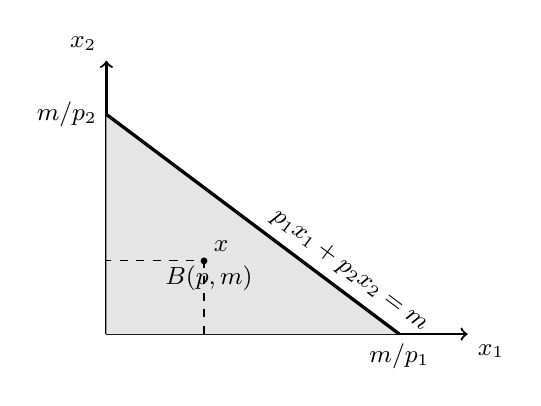
\begin{tikzpicture}[scale=0.62]
  \draw[->,thick] (0,0) -- (7.4,0) node[below right] {\small $x_1$};
  \draw[->,thick] (0,0) -- (0,5.6) node[above left] {\small $x_2$};
  % 预算集阴影
  \fill[gray!20] (0,0) -- (6,0) -- (0,4.5) -- cycle;
  \draw[very thick] (6,0) -- (0,4.5) node[midway,above right,sloped] {\small $p_1x_1+p_2x_2=m$};
  \node[below] at (6,0) {\small $m/p_1$};
  \node[left] at (0,4.5) {\small $m/p_2$};
  \node at (2.1,1.15) {\small $B(p,m)$};
  \draw[dashed] (2,0) -- (2,1.5) -- (0,1.5);
  \fill (2,1.5) circle (2pt) node[above right] {\small $x$};
\end{tikzpicture}
\caption{二维预算集：截距、斜率与可行域}
\end{figure}
\figexplan{浅灰三角区域（含边界）即预算集 $B(p,m)$，其斜边为预算线 $p_1x_1+p_2x_2=m$，在两轴上的截距分别为 $m/p_1$ 与 $m/p_2$，斜率为 $-p_1/p_2$。虚线给出可行束 $x$ 的坐标读数。价格比决定斜率（机会成本），收入决定截距。}

\begin{proposition}[预算集的基本性质]
设 $p\in\R_{++}^{L}$，$m\ge 0$，则 $B(p,m)$ 是非空、有界、闭且凸的集合。
\end{proposition}

\begin{proof}
\textbf{非空}：$0\in B(p,m)$，因 $p\cdot 0=0\le m$。
\textbf{有界}：对 $x\in B(p,m)$，由 $p_l>0$ 与 $x_l\ge 0$ 得 $x_l\le m/p_l$，故 $\lVert x\rVert\le \sqrt{L}\,\max_l(m/p_l)$。
\textbf{闭}：$B(p,m)$ 是闭集 $\{x:p\cdot x\le m\}$ 与闭集 $\R_+^{L}$ 的交，闭集的交仍闭。
\textbf{凸}：任取 $x,y\in B(p,m)$ 与 $\lambda\in[0,1]$，记 $z=\lambda x+(1-\lambda)y$。则 $z_l=\lambda x_l+(1-\lambda)y_l\ge 0$，且
\[
p\cdot z=\lambda\,(p\cdot x)+(1-\lambda)(p\cdot y)\le \lambda m+(1-\lambda)m=m,
\]
故 $z\in B(p,m)$。
\end{proof}

\begin{remark}
这个命题值得逐字咀嚼：价格严格为正、收入非负、数量非负——三条看似平淡的假设，恰好保证了下一节要用到的“紧且凸”结构。每一条经济假设都在数学上有明确后果。
\end{remark}

\subsection{映射：从方案到数}

\begin{definition}[函数]
设 $X,Y$ 为两个集合。\emph{函数}（映射）$f:X\to Y$ 是一个规则，使每个 $x\in X$ 对应\emph{唯一}的 $y\in Y$，记 $y=f(x)$。$X$ 称\emph{定义域}，$Y$ 称\emph{值域}（陪域）。
\end{definition}

函数有三要素：定义域、值域、对应规则。三者有一个不同，就是不同的函数。

\begin{definition}[单射、满射、双射]
$f:X\to Y$ 称为\emph{单射}，若 $f(x_1)=f(x_2)\Rightarrow x_1=x_2$；称为\emph{满射}，若对每个 $y\in Y$ 都存在 $x\in X$ 使 $f(x)=y$；既是单射又是满射则称\emph{双射}。
\end{definition}

\begin{example}[效用是一种映射]
在经济学中，映射可以把消费束映为一个实数：
\[
u:X\to\R .
\]
例如 Cobb–Douglas 效用 $u(x_1,x_2)=x_1^{\alpha}x_2^{1-\alpha}$（$0<\alpha<1$），或完全替代效用 $u(x_1,x_2)=a x_1+b x_2$。
\end{example}

这里的 $u(x)$ 是对偏好排序的\emph{数值表示}，而不是方案本身。把方案映到实数，目的是把“更好”转化为可运算的序关系——但这一步骤需要行为假设（理性偏好，见第 5 节），并不等于我们观察到了某种内在的心理单位。

\begin{remark}[效用的序数性]
若 $u$ 表示某偏好，则对任意严格递增变换 $g:\R\to\R$，复合函数 $v=g\circ u$ 表示\emph{同一个}偏好，因为 $u(x)\ge u(y)\iff v(x)\ge v(y)$。所以效用只承载\emph{排序}信息：两个消费束谁更好有意义，“好多少”没有意义。这一“序数性”将在第 6 节评价福利比较时再次出现。
\end{remark}

\notehead{本节要点}
\begin{itemize}
  \item 集合语言：$\in,\subseteq,\cup,\cap,\setminus,(\cdot)^{c},\times,\varnothing$；集合相等用双向包含证明；
  \item $\R^{L}$ 中的开/闭、有界、紧、凸——它们分别对应哪些经济含义；
  \item $B(p,m)=\{x\in\R_+^{L}:p\cdot x\le m\}$ 非空、有界、闭、凸（四条逐条可证）；
  \item 函数三要素；效用映射 $u:X\to\R$ 是序数概念。
\end{itemize}
